% Figure from MATH 591 notes, section 31. Compile with the notes preamble.
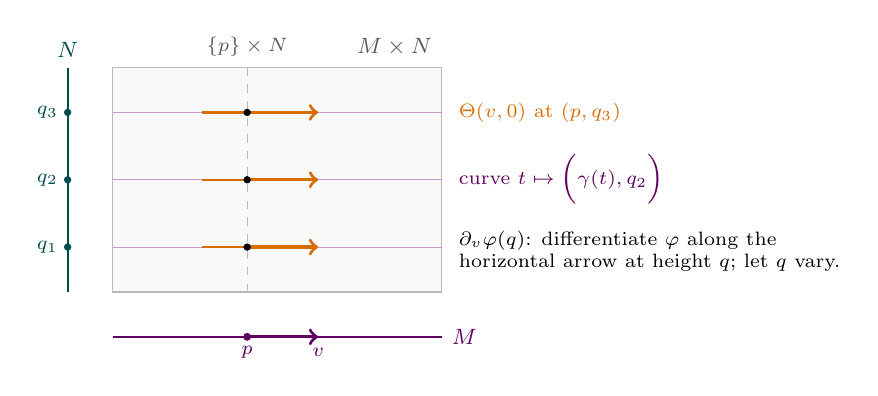
\begin{tikzpicture}[scale=0.95]
\fill[gray!5] (0,0) rectangle (4.4,3); \draw[gray!55] (0,0) rectangle (4.4,3);
\node[font=\footnotesize, gray!70!black, anchor=south east] at (4.4,3.02) {$M \times N$};
\draw[violet!75!black, thick] (0,-0.6) -- (4.4,-0.6) node[right, font=\footnotesize] {$M$};
\draw[teal!60!black, thick] (-0.6,0) -- (-0.6,3) node[above, font=\footnotesize] {$N$};
\draw[gray!55, dashed] (1.8,0) -- (1.8,3);
\node[font=\scriptsize, gray!70!black, anchor=south] at (1.8,3.02) {$\{p\} \times N$};
\foreach \y/\lab in {0.6/q_1, 1.5/q_2, 2.4/q_3} {
  \draw[violet!40] (0,\y) -- (4.4,\y);
  \draw[orange!85!black, thick] (1.2,\y) -- (2.4,\y);
  \draw[->, very thick, orange!85!black] (1.8,\y) -- (2.75,\y);
  \fill (1.8,\y) circle (1.4pt);
  \fill[teal!60!black] (-0.6,\y) circle (1.4pt) node[left, font=\scriptsize] {$\lab$};
}
\node[font=\scriptsize, anchor=west, orange!85!black] at (4.5,2.4) {$\Theta(v, 0)$ at $(p, q_3)$};
\node[font=\scriptsize, anchor=west, violet!75!black] at (4.5,1.5) {curve $t \mapsto \big(\gamma(t), q_2\big)$};
\fill[violet!75!black] (1.8,-0.6) circle (1.5pt) node[below, font=\scriptsize] {$p$};
\draw[->, very thick, violet!75!black] (1.8,-0.6) -- (2.75,-0.6) node[below, font=\scriptsize] {$v$};
\node[font=\scriptsize, anchor=west, align=left] at (4.5,0.55) {$\partial_v\varphi(q)$: differentiate $\varphi$ along the\\ horizontal arrow at height $q$; let $q$ vary.};
\end{tikzpicture}
